\documentclass{article}
\usepackage[utf8]{inputenc}
\usepackage{pgfplots}
\pgfplotsset{width=10cm,compat=1.9}
\usepackage{amsmath,amssymb,amsthm}
\usepackage{graphicx}
\usepackage{float}
\usepackage{mathtools}
\usepackage{xcolor}
\usepackage[margin=1in]{geometry}
\usepackage{blindtext}
\usepackage{hyperref}
\hypersetup{
    colorlinks=true,
    linkcolor=blue,
    filecolor=magenta,      
    urlcolor=cyan,
    pdftitle={Overleaf Example},
    pdfpagemode=FullScreen,
    }
\usepackage[slovene]{babel}


%\usepackage{helvet}
%\renewcommand{\familydefault}{\sfdefault}

\newcounter{example}[section]
\newenvironment{example}[1][]{\refstepcounter{example}\par\medskip
   \noindent \textbf{Naloga~\theexample. #1} \rmfamily}{\medskip}

\newtheorem*{zgled}{Zgled}

\title{Polinomi in racionalne funkcije}
\author{Bor Bregant}
\date{\vspace{-5ex}}

\begin{document}

\maketitle


\section{Polinomi}

Polinom je funkcija $p(x)=a_n x^n+a_{n-1}x^{n-1}+\ldots+a_1 x+a_0$, kjer je $a_n\neq 0$. $n$ imenujemo stopnja polinoma, $a_0$ prosti člen, $a_n$ vodilni koeficient, $a_0,\ldots,a_n$ pa koeficienti polinoma $p$.\\
$p(x)=0$ imenujemo ničelni polinom.\\
Polinoma sta enaka, če imata enako stopnjo in enake koeficienti pri enakih potencah $x$.

\begin{zgled}
    \textdagger Zapiši stopnjo, koeficiente in vrednost pri $x=2$ za $p(x)=3x^4-2x^3+11x-7$\\
    \textdagger Zapiši polinom druge stopnje, če veš, da je $p(8)=6, p(2)=0$ in $p(0)=4$. Izračunajmo še njegovo vrednost za x=1.
\end{zgled}

\begin{example}
    NALOGE 1, 2, 3, \fbox{7}, 8
\end{example}

\textbf{Množenje polinoma s številom, seštevanje, odštevanje in množenje polinomov:}
\begin{zgled}
    Pomnožimo polinom $r(x)=2x^4+3x^2-8x+5$ s številom $\frac{3}{2}$.\\
    Seštejmo polinoma $p(x)=3x^4+7x^3-4x^2+6$ in $q(x)=7x^5+2x^3+7x^2+8x-5$. Za isti primer izračunajmo še $q(x)-p(x)$.\\
    Zmnožimo polinoma $p(x)=x^2+1$ in $q(x)=x^3-4x^2+6$.
\end{zgled}
Za množenje polinomov velja $st(p\cdot q)=st(p)+st(q)$, komutativnost in asociativnost.\\

\textbf{Deljenje polinomov:}\\

Za vsak polinom $p$ stopnje $n$ in polinom $q$ stopnje $m$ $(n\geq m)$ obstajata natanko določena polinoma $k$ in $r$, da velja $p(x)=k(x)q(x)+r(x)$. $k$ imenujemo kvocient in je stopnje $n-m$, $r$ pa ostanek in je nižje stopnje kot $q$.

\begin{zgled}
    Delimo $(x^2+x-3):(x+3)$\\
    Delimo polinom $p(x)=3x^4+5x^3-4x^2+7$ s polinomom $q(x)=x^2+2x-1$.
\end{zgled}
\begin{zgled}
    Če polinom $p(x)=x^5-3x^3-5x$ delimo z neznanim polinomom $q$ dobimo kvocient $k(x)=x^3+x^2-3x-4$ in ostanek $r(x)=-6x+4$. Določimo $q$.
\end{zgled}

\begin{example}
    NALOGA 16ab, 17a, 20a, 23, 27b,c,e,g, \fbox{28a}c, 30, 36
\end{example}


\textbf{Hornerjev algoritem} - Postopek za deljenje polinoma z linearnim polinomom.\\
Velja tudi, da je ostanek pri deljenju polinoma $p$ z linearnim polinomom $x-c$ enak vrednosti $p$ pri $x=c$.

\begin{zgled}
    S Hornerjevim algoritmom delimo $3x^5-4x^4-7x^2+3x-4$ z $x-2$. Preverimo še, da je ostanek res enak vrednosti $p(2)$.\\
    Enaka naloga $(x^3-4x^2+6x-7):(x-3)$, $(2x^5-2x^4-13x^3+7x+6):(x+1)$.\\
    Zapiši vrednost $p(x)=x^4-3x^3+2x^2+2x-4$ v točki $x=i$.\\
    S hornerjevim algoritmom pokažimo, da je polinom $p(x)=x^4+8x^3+6x^2-13x-2$ deljiv s polinomom $q(x)=x^2+x-2$.
\end{zgled}

\begin{example}
    NALOGE 45, 46, 48b
\end{example}

\subsection{Ničle polinoma: $p(x)=0$}

Razstavimo, kjer si lahko pomagamo s hornerjem. Ko pridemo do kvadratne člena v vietovim pravilom ali kvadratno formulo. Rezultat je ničelna oblika $p(x)=a(x-x_1)^{k_1} \cdots (x-x_l)^{k_l}$
$c$ je ničla polinoma $p$ natanko tedaj, ko je $p$ deljiv s polinomom $x-c$. Pri deljenju si pomagamo s Hornerjem!

\begin{zgled}
    Preverimo, da je $x=-2$ ničla polinoma $p(x)=2x^4+3x^3-7x^2+x+22$.\\
    Razcepimo izraz $x^3-7x+6$ kot produkt linearnih faktorjev, če vemo da je eden od faktorjev $x+3$.\\
    Izračunajmo vse ničle $f(x)=x^4-x^2$.\\
    Razcepimo izraz $3x^3-20x^2+42x-20$, če vemo, da je ena faktor $x-\frac{2}{3}$.
\end{zgled}

Polinom stopnje $n$ ima natanko $n$ (kompleksnih) ničel štetih z večkratnostjo. Kompleksne ničle nastopajo v konjugiranih parih.

\begin{zgled}
    (a) Zapišimo polinom tretje stopnje, ki ima prosti člen enak $-2$ in ima enkratno ničlo 1 in dvakratno ničlo $\frac{1}{2}$.\\
    (b) Poiščimo ničle polinoma $p(x)=x^4-4x^3-2x^2+12x+9$, če vemo, da je $(-1)$ dvakratna ničla.\\
    (c) Zapišimo polinom tretje stopnje, ki ima ničli $2+i$ in $1$, pri $x=0$ pa vrednost $\frac{1}{2}$.\\
\end{zgled}

\textbf{Kandidati za ničle:} Kandidati za celoštevilske ničle polinoma so delitelji prostega člena. Kandidati za racionalne ničle polinoma so oblike $\frac{c}{d}$, kjer $c$ deli prosti člen, $d$ pa vodilni koeficient.

\begin{zgled}
    Izračunajmo vse ničle polinoma $p(x)=12x^4-20x^3+7x^2+2x-1$.
\end{zgled}

\begin{example}
    NALOGE 53, 56, 58, 68, 74, \fbox{92ab}, 93a, 95a, \fbox{97ab}, 99ab
\end{example}

\begin{zgled}
    Zapiši rešitve enačbe $x^3-6x^2=-11x+6$ in $x^3+x^2=5x+2$.
\end{zgled}


\subsection{Graf polinoma}

Začetna vrednost $p(0)$.\\
Če je ničla lihe stopnje (enkratna, trikratna, ...) polinom v ničli spremeni predznak. Če je ničla sode stopnje se predznak ne spremeni.

\begin{figure}[H]
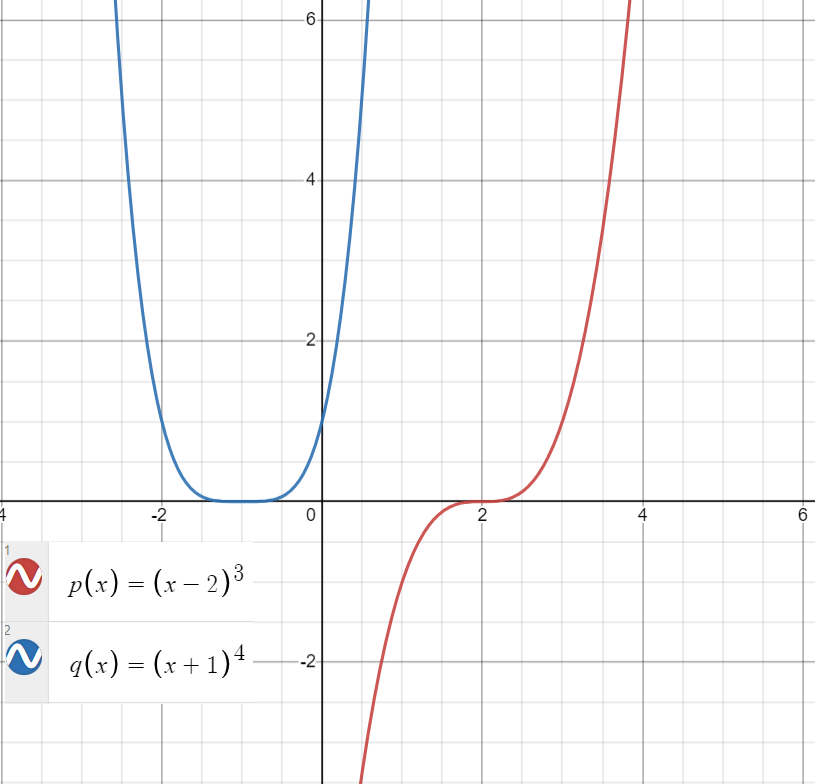
\includegraphics[width=0.6\textwidth]{polinomi.grafi.png}
\centering
\caption{Grafa funkcij z ničlo \textcolor{red}{lihe} in \textcolor{blue}{sode} stopnje.}
\centering
\end{figure}

\textbf{Obnašanje grafa v $\pm \infty$:}

Če $a_n>0$, gre graf proti $\infty$ v $+\infty$. Če $a_n<0$, gre graf proti $\infty$ v $-\infty$.\\
Če je $n$ sod, se graf obnaša ''podobno'' v $\infty$ in $-\infty$. Če $n$ lih se obnaša ''obratno''.

\begin{figure}[H]
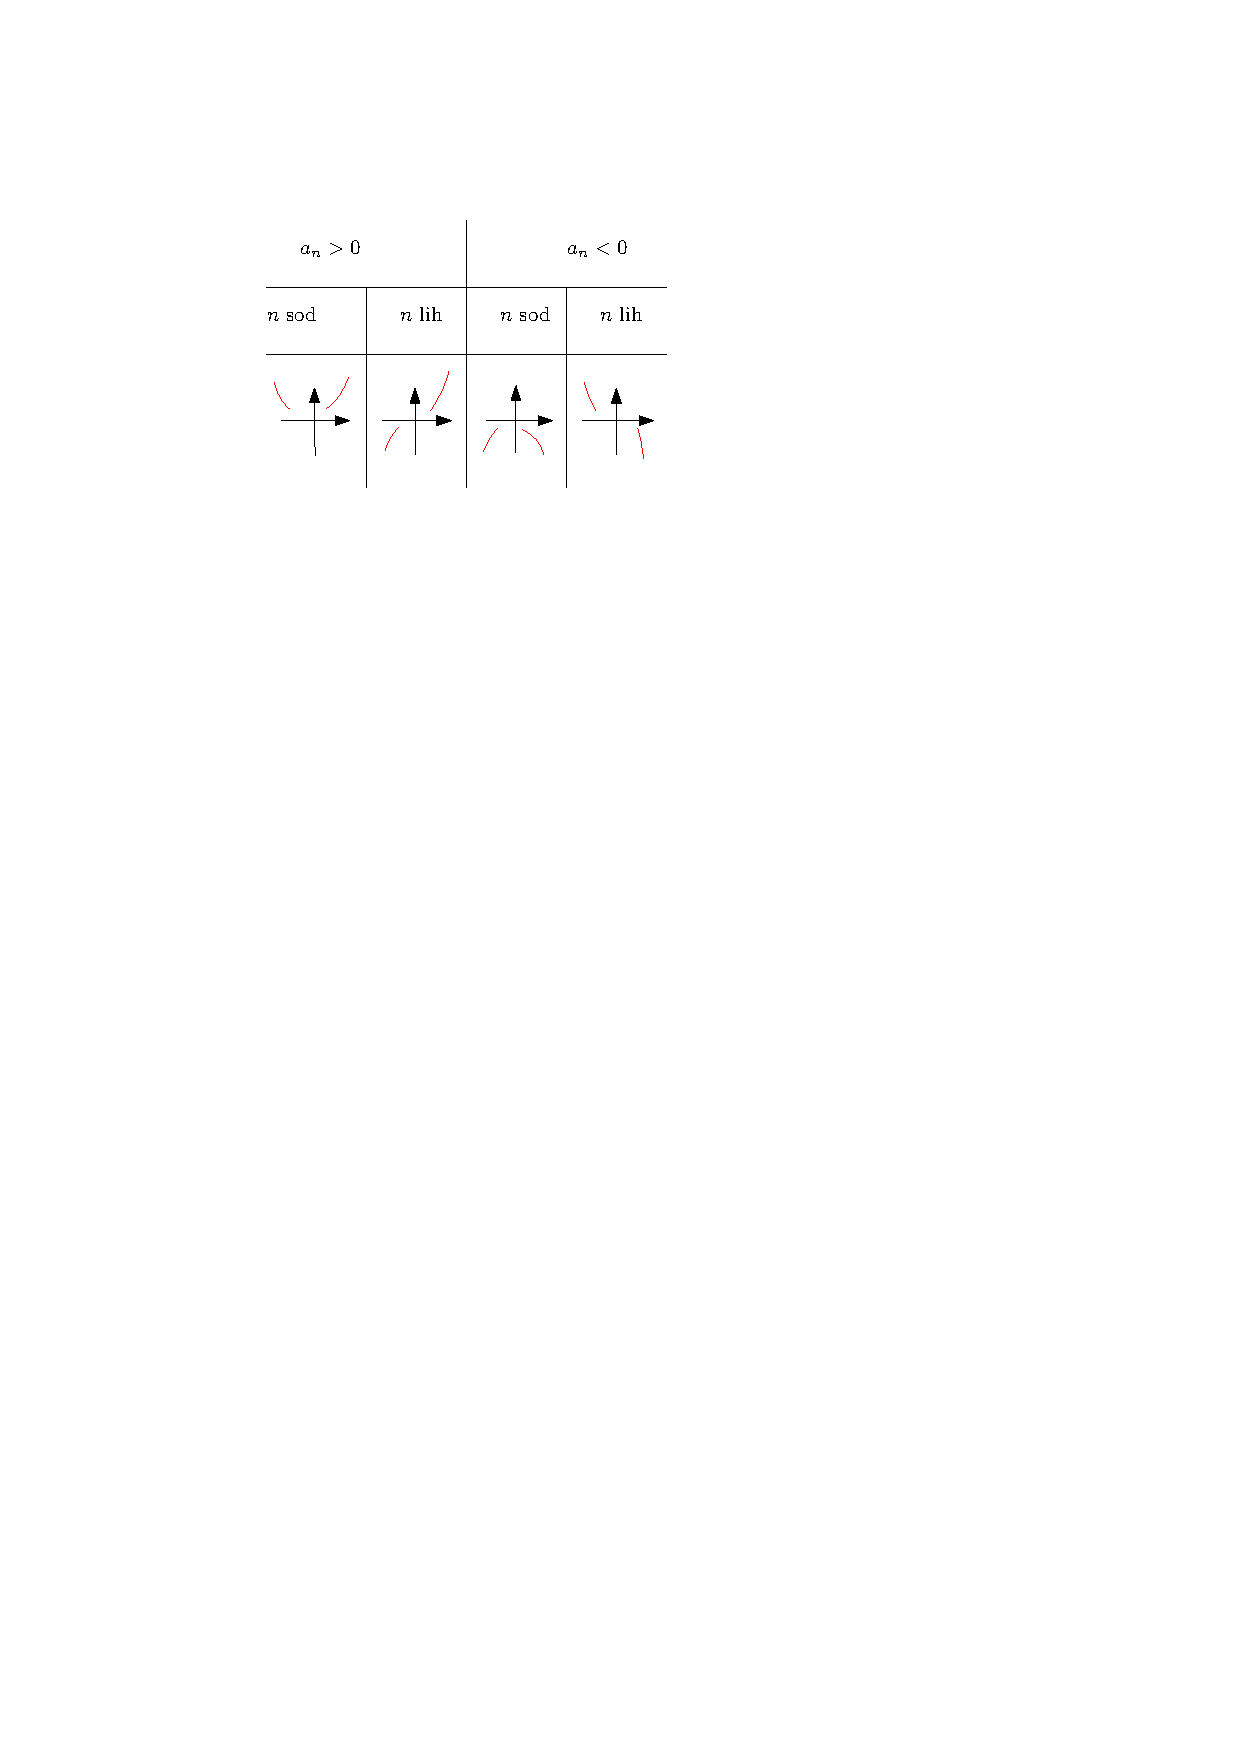
\includegraphics[width=0.5\textwidth]{polinom.infty.pdf}
\centering
\end{figure}


\begin{zgled}
    Narišimo graf polinoma $p(x)=x^3-3x+2$ in grafe $|p(x)|,p(|x|),2p(x),p(2x),p(x-2),p(x)-2$.\\
    Resimo se neenačbo $p(x)\geq0$.\\
    Nariši še grafe $p(x)=x^4-4x^2$, $p(x)=x^3+x^2-5x+3$, $p(x)=-(x+1)(x-1)^2$\\
    Zapiši predpis za narisan graf - Enojna ničla $-2$, dvojna $1$, zacetna vrednost $3$
\end{zgled}

\begin{example}
    NALOGE 116ab, 119, 120, 124, \fbox{127}, 130, 144a,č, 154a
\end{example}

\subsection{Bisekcija}

Metoda za iskanje ničel. Če je $f$ realna zvezna funkcija na $[a,b]$ in je v $a$ in $b$ različno predznačena obstaja $c\in (a,b)$, da $f(c)=0$. V vsakem koraku zamenjamo eno točko intervala z razpoloviščem le tega, torej se v vsakem koraku napaka razpolovi.
\begin{zgled}
    Približno poiščimo iracionalno ničlo za $p(x)=x^5+2x-1$ na $[0,1]$.
\end{zgled}


\section{Racionalne funkcije}

$f(x)=\frac{p(x)}{q(x)}$, kjer sta $p$ in $q$ polinoma. Ničle $f$ = ničle $p$, $D_f=\mathbb{R}\backslash\{x|q(x)=0\}$. Ničle imenovalca imenujemo poli.

\begin{zgled}
    Določimo $D_f, D_g, g+f, g\cdot f$, ničle in pole $f$ in $g$ za $f(x)=\frac{3x-2}{x^2-4}$ in $g(x)=\frac{3}{x}$
\end{zgled}

\begin{example}
    NALOGE 168a,b,c, 170a
\end{example}

\subsection{Graf racionalne funkcije}

Ničle podobno kot pri polinomih.\\
V polih ima graf navpično asimptoto. Če je pol lihe stopnje graf spremeni predznak. Če je pol sode stopnje graf ne spremeni predznaka.\\
Lahko si pomagamo z vmesnimi točkami npr. začetno vrednostjo
\begin{figure}[H]
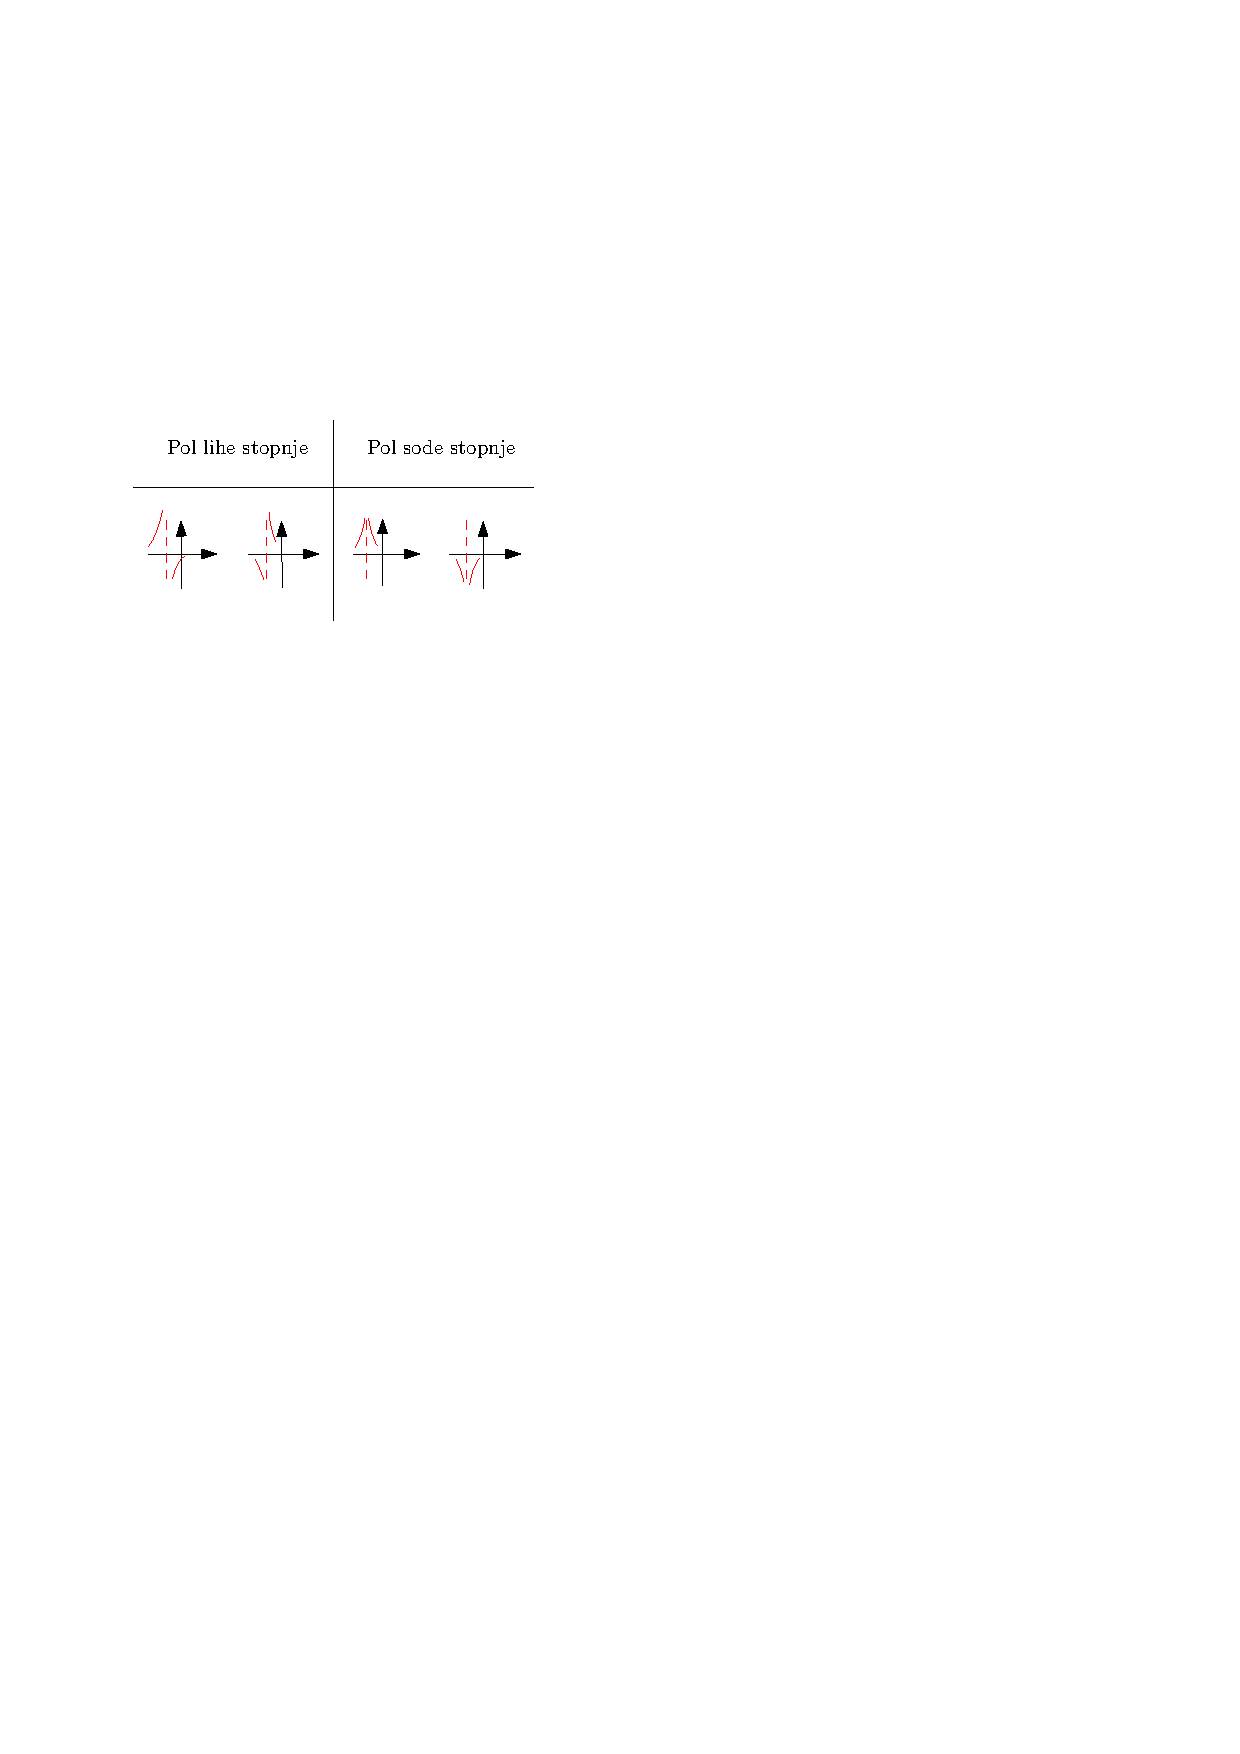
\includegraphics[width=0.7\textwidth]{racionalna.poli.pdf}
\centering
\end{figure}

\textbf{Obnašanje grafa v $\pm \infty$:}

\[f(x)=\frac{p(x)}{q(x)}=\frac{a_nx^n+\ldots+a_0}{b_mx^m+\ldots+b_0}\xrightarrow{x\to\pm\infty}\frac{a_nx^n}{b_mx^m}\]
\begin{itemize}
    \item \textbf{$n<m$}: Vodoravna asimptota $y=0$.
    \item \textbf{$n=m$}: Vodoravna asimptota $y=\frac{a_n}{b_n}$.
    \item \textbf{$n>m$}: Delimo $p:q$. Celi del rešitve je funkcija kateri se približujemo. V točkah, kjer je ostanek enak $0$, pa to (krivuljno) asimptoto sekamo (tudi za $n=m$).
\end{itemize}

\begin{zgled}
    Narišimo grafe\\
    (a) $f(x)=\frac{x+3}{x^2-4x+4}$ \qquad (b) $f(x)=\frac{2x+6}{3x-3}$ \qquad (c) $f(x)=\frac{x^2+4x+4}{x+3}$\\
    Zapiši predpis racionalne funkcije, ki ustreza grafu ...
\end{zgled}

\begin{example}
    175a,b, 183 vse, \fbox{189a,b}, \fbox{193a,b}.
\end{example}

\subsection{Racionalne enačbe in neenačbe}

Vse damo na eno stran (pri neenačbi to storimo z odštevanjem ne množenjem!). V enačbi so rešitve ničle novega grafa, v neenačbi pa $x$, kjer je graf nad oz. pod $x$ osjo.

\begin{zgled}
    Reši enačbi $\frac{x+1}{x-4}=6$ in $\frac{2x}{x-1}+\frac{1}{x-3}=\frac{2}{x^2-4x+3}$.
\end{zgled}
\begin{zgled}
    V kateri točki se sekata grafa funkcij $f(x)=\frac{x-3}{x+2}$ in $g(x)=\frac{x+1}{x+3}$.
\end{zgled}
\begin{zgled}
    Vsota števila in dvakratnika njegovega obratnega števila je $\frac{9}{2}$. Katero število je to?
\end{zgled}
\begin{zgled}
    Rešimo neenačbo $\frac{x+2}{2x+2}\geq\frac{x-2}{x+1}$.
\end{zgled}
\begin{zgled}
    \textcolor{red}{Na katerem intervalu je $f(x)=\log(\frac{x}{x+2}-\frac{1}{x})$ pozitivna?}
\end{zgled}
\begin{zgled}
    Zapiši ničle, pole, nariši graf za $f(x)=\frac{3x^2+10x+3}{x^3+2x^2-7x+4}$. Kje $f$ zavzame vrednosti $-\frac{1}{3}$.
\end{zgled}


\begin{example}
    NALOGE 195a,b, 200a, 201a,d, 206, 207
\end{example}



\end{document}